\lfoot{Autor: Raphael Simsek}
\subsection{Analyse und Verbesserung des Fahrstils}

\todo{Bezug auf wie sie in der Graphik unten erkennen können, auf wie sie in Abb. 1 erkennen können ändern}
\todo{Sätze mit max. 1 Beistrich formulieren}
\todo{Reihenfolge der Paragraphen ändern}
Häufig kann nicht immer der Fahrlehrer einem Fahrschüler einen nachhaltigen oder wünschenswerten Fahrstil näher bringen. Dies ist nämlich oft ein zeitintensiver Prozess ist. Aus diesem Grund wurden sich Gedanken dazu gemacht, wie man diese Situation verbessern kann.

\subsubsection{Was soll umgesetzt werden?}
\begin{itemize}
	\item Echtzeit Messung und Errechnung der Beschleunigungskräfte, des Schadstoffausstoßes und eines Schaltvorschlags mittels der OBD-II Schnittstelle
	\item Darstellung des Schaltvorschlags, Fahrkomforts und Schadstoßes in einer Android Applikation
	\item retrospektive Analyse der Fahrkomfortanalyse einer Fahrt
	\item retrospektive Analyse des errechneten Verbrauchs einer Fahrt
	\item Darstellung der retrospektiven Analyse mittels einer Web-Applikation
	\item Sharing Möglichkeiten für die Analyse seiner Fahrt
	\item Realisierung eines Car-PC
\end{itemize}

\subsubsection{Sharing}
Am Beginn des Projektes wurde nach bereits bekannten Systemen gesucht, um seinen Fahrstil nachhaltig zu verbessern. Bei dieser Suche stach die Verbreitung von Apps mit \textit{Sharing}-Funktion heraus. Es gibt nämlich bereits in vielen anderen Bereichen Apps, die sich das \textit{Sharing}-Prinzip zu Nutze machen und damit äußerst erfolgreich Ihre Kunden zu einer Veränderung Ihrer Gewohnheiten bringen \cite{SIMR.CH1-fahrstil-analyse.GewohnheitenLoslassen}. Eines der bekanntesten österreichischen Beispiele ist das App-System von Runtastic \cite{SIMR.CH1-Fahrstil-Analyse.BusinessplanRuntastic}.
Nur im Bezug auf das Autofahren konnte kein derartiges System  gefunden werden.

Zu Beginn des Diplomprojektes gab es folglich keine Möglichkeiten für verbesserungswillige Autofahrer ihren Fahrstil zu verbessern und dies dann sogar zu teilen. 
\newpage
\paragraph{Peer-Pressure} 
\begin{wrapfigure}{r}{0.6\textwidth}\centering
    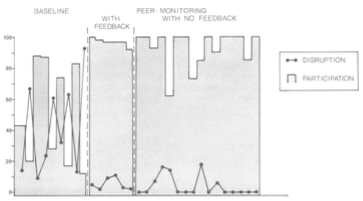
\includegraphics[width=0.6\textwidth]{images/peerPressure}
    \caption{Verhaltensanalyse von Kindern bei gegenseitigem Monitoring \cite{SIMR.CH1-fahrstil-analyse.PeerPressure}} \label{Fig:imgPeerPressure}
\end{wrapfigure}
Das Teilen der Fahrstilanalyse trägt durch \textit{Peer-Pressure}  dazu bei, dass die Nutzer andere Nutzer überbieten möchten und so ihren eigenen Fahrstil verbessern. Diese Theorie bestätigt eine Studie, bei der sich Schüler gegenseitig beobachten. Die Studie zeigt, dass von gleichgesinnten umgebene und überwachte Schüler (hier Social Network) sich selbst angepasster verhalten und sich auf Ihre Vernunft besinnen \cite{SIMR.CH1-fahrstil-analyse.PeerPressure}. Es würden sich Fahrer folglich genauso vernünftiger fahren, wie sich die Schüler in dieser Studie verhalten haben.

Bei der Evaluierung des Project Scope fiel uns besonders auf, dass eine Analyse-Funktion für die nachhaltige Verbesserung des Fahrstils behilflich sein könnte. Es wurde für diese Analyse evaluiert, welche Funktionalitäten am Wichtigsten sind, wobei diese auch innerhalb der Diplomarbeit realisierbar sein sollten.

\subsubsection{Fahrkomfortanalyse}
Eine Analyse des Fahrstils, nach Parametern der Fahrgastbequemlichkeit, ist gar nur bei Sportwagen und Fahrzeugen, die für den Rennbetrieb gedacht sind, verbaut. Hierbei ist anzumerken, dass bei derartigen Fahrzeugen die Funktionalität nicht für das frühzeitige Verbessern des Fahrstils eines Fahrers verwendet wird, sondern für die Optimierung von Rundenzeiten auf einer Rennstrecke oder schier für das Ausreizen des Möglichen.

\begin{figure}[!htb]\centering
	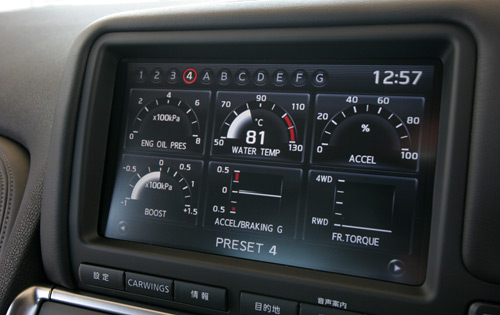
\includegraphics[width=0.6\textwidth]{images/gtrMultifunc}
	\caption{Analyse Möglichkeiten bei einem Nissan GT-R (R35) \cite{SIMR.CH1-Fahrstil-Analyse.GTRMultifunc}}\label{Fig:imgGTR}
\end{figure}

Im Kontrast zu bisher etablierten Möglichkeiten ist die Anzeige der Fahrgastbequemlichkeit anhand fundamental anderen Parametern aufgebaut. Sie soll dem Fahrer aufzeigen welche Kurven dieser zu schnell durchfahren hat. Als Maß für die Bequemlichkeit wird dabei die Beschleunigungskraft in g [Kraft/Masse] herangezogen. Genauere Ausführungen zu diesem Thema, können unter Kapitel 3.5 - Fahrkomfortanalyse gefunden werden.

\subsubsection{Schaltvorschlag}
Der bisherige Schaltvorschlag in einem Auto ist, insbesondere bei kostengünstigeren Fahrzeugen, oft äußerst simpel gehalten, wobei ab einer gewissen Drehzahl die darauffolgenden Gänge vorgeschlagen werden oder auf den Normzyklus optimiert wird. \cite{SIMR.CH1-Fahrstil-Analyse.Schaltempfehlung} 
\paragraph{Normzyklus}
Der Normzyklus ist insbesondere aufgrund des VW-Skandals bekannt geworden. Es erkennt die Motorsteuerung nämlich, wenn ein Abgastest gefahren wird. Dieser wird in der Fachsprache als Normzyklus bezeichnet wird \cite{SIMR.CH1-fahrstil-analyse.Normzyklus}. Der \textit{modifizierte neue europäische Fahrzyklus (MNEFZ)} ist der Normzyklus, der innerhalb der EU verwendet wird um den Normverbrauch eines Fahrzeuges zu errechnen. Dieser umfasst insgesamt 1180 Sekunden, wovon 780 Sekunden unter Stadtbedingungen und 400 Sekunden über Land gefahren werden. Er wird hauptsächlich aufgrund der Tricks, die Autohersteller verwenden dürfen, kritisiert. Herstellerangaben werden in Europa nämlich selten hinterfragt \cite{SIMR.CH1-fahrstil-analyse.MNEFZ}. Besonders in den USA mussten dafür die Automobilhersteller hohe Entschädigungen zahlen (cite: http://www.spiegel.de/auto/aktuell/geschoente-verbrauchswerte-bmw-muss-angaben-beim-mini-korrigieren-a-999742.html#ref=plista)
\paragraph{Carnot-Prozess}
Der Motorwirkungsgrad nach dem Carnot-Prozess, wird für den Schaltvorschlag meist nicht verwendet. Der Carnot-Prozess beschreibt die Errechnung des \textit{theoretisch möglichen} Motorwirkungsgrad, ohne hinzuziehen von Reibung, Temperatur und anderen natürlichen Einflussgrößen. \cite{SIMR.CH1-Fahrstil-Analyse.CarnotWirkungsgrad} Genauere Ausführungen zu diesem Thema können im Kaptiel 2.1.2 - Thermodynamik gefunden werden. 

\subsubsection{Schadstoffausstoß}
Eine Live-Messung von \ce{CO2} Werten während der Fahrt ist zumeist eine Schätzung, welche durch den Bordcomputer durchgeführt wird und noch bei wenigen Modellen Einsatz findet. Echte Grenzwerte oder gar eine Analysefunktionalität gibt es in dieser Hinsicht aber nicht. Die \ce{CO2} Werte werden in Zukunft allerdings noch weitaus relevanter, weil, wie im folgenden Kapitel (1.2 - Umweltbelastung durch \ce{CO2} Ausstoß) ausführlich beschrieben, bis 2020 versucht wird einen Durschnittsaustoß von 95 g/km zu erzielen. \cite{SIMR.CH1-Fahrstil_Analyse.EUVerordCO2} Deshalb ist uns diese Funktionalität besonders im Bezug auf Zukunftssicherheit bei bisherigen Bordcomputern als fehlend aufgefallen.

\subsubsection{Analysefunktion}
Besonders für Fahranfänger kann solch eine Funktionalität von großer Hilfe als lernunterstützendes Medium sein, da momentan ein Fahrschüler nach seiner Fahrstunde nur ein subjektives Feedback seines Fahrlehrers bekommt. Wie ließe sich eine solche Lernunterstützung also umsetzen?
Man könnte dem Fahrschüler am Ende der Fahrstunde eine faktenbasierte Übersicht über seine Leistung während der Fahrstunde geben, welche er dann auch mitnehmen kann und wodurch dieser weiß worauf er bei seiner nächsten Übungsmöglichkeit achten sollte. Diese Übersicht ist sowohl ausgedruckt, als auch, wie unterhalb erkennbar, mittels unserer Webapplikation denkbar.

\todo{Insert image of web application}
%\begin{figure}[!htb]\centering
%	\includegraphics[width=0.6\textwidth]{images/}
%	\caption{Beispiel Analyse mittels unserer Webapplikation}\label{Fig:imgWebapp}
%\end{figure}

Besonders Fahranfänger und Fahrer mit Umweltinteresse könnten die entwickelte Analysefunktionalität gerne nutzen wollen. Die Analysefunktionalität soll besonders für die Zielgruppe eines Fahranfängers aufzeigen, wo der Verbrauch, die Kurvenbeschleunigung (G-Kraft) und die Drehzahl besonders hoch war, damit sich der Fahranfänger oder der interessierte Kunde zukünftig verbessern kann. Da uns noch kein derartiges System bekannt war, wurde ebenfalls evaluiert ob die Möglichkeiten einer retrospektiven Fahranalyse durch Anbauteile oder Zubehör bereits realisierbar sind.

\paragraph{Car - PC}
Bei der Evaluierung konnte ein Projekt gefunden werden, welches die gelieferten Daten nur in Echtzeit per Computer auslesbar macht. Die Daten werden aber sofort verworfen, weshalb keine retrospektive Analyse mehr möglich wäre. Überdies ist die Programmierung in einer anderen Programmiersprache umgesetzt, weshalb man dieses Projekt keinesfalls auf Android portieren könnte. Das Projekt ist außerdem weitaus teurer (geschätzt €300,-) als von uns gewünscht, denn es wurde überlegt bis zu welchem Preis man sich ein solches Zubehör, auch als normaler Anwender leisten würde, wobei für uns €100,- als Abgrenzung feststand. Daher wurden Überlegungen angestellt, wie man die Idee eines solchen Projektes massentauglicher machen kann und dabei bei geringen Kosten dem Nutzer ein wünschenswertes Erlebnis bieten kann. \cite{SIMR.CH1-Fahrstil-Analyse.LowBudgetCarPC} Dieses Projekt hat uns also geholfen in der Defintionsphase des Projektes Anpassungen vorzunehmen, da es bereits einen Maßstab gab, was im Bereich des Möglichen liegt. Weitere Ausführungen zu dieser Thematik sind unter Kapitel 2.2 - Hardware und Sensorik auffindbar.

Es gibt bisher bei konkurrierenden Echtzeit-Anzeigen (wie. z.B. Torque Pro \cite{SIMR.CH1-Fahrstil-Analyse.TorquePro}) noch keine, wie beschriebene, Analysefunktionalität. Deshalb würde die Analysefunktionalität für einen Autofahrer ein noch nicht etabliertes Produkt darstellen.

\begin{figure}[!htb]\centering
	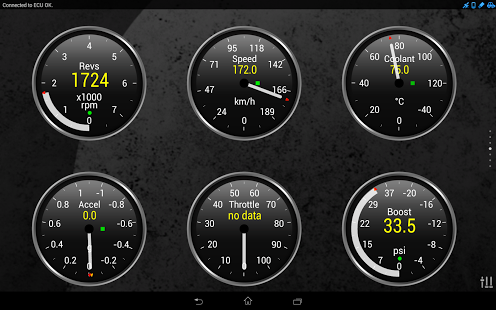
\includegraphics[width=0.6\textwidth]{images/torquePro}
	\caption{Möglichkeiten mit der kostenpflichtigen Torque App  und der OBD Schnittstelle \cite{SIMR.CH1-Fahrstil-Analyse.TorquePro}}\label{Fig:imgGTR}
\end{figure}

Gerade diese Funktionalität würde aber von Fahranfängern benötigt werden um frühzeitig und selbstständig Fehler ihres Fahrstils zu erkennen und auszubessern zu können. Insbesondere konnten wir, unter anderem anhand unserer Erfahrungen, feststellen, dass das Schalten und das gleichmäßige und verbrauchsarme Fahren für viele Fahranfänger eine Herausforderung darstellt. Durch eine Analysefunktion könnten motivierte Fahranfänger Anfangsschwieriegkeiten schneller ablegen und die schlechten Angewohnheiten würden sich nicht im  Gedächtnis eines Fahranfängers verankern. Stattdessen es würden sich, unter regelmäßiger Verwendung der Applikation, bei motivierten Fahrern nur positive Charakteristika gemerkt werden, wie bei regelmäßigem Fahren mit einer erfahrenen Person merken konnten.

Eine Analysefunktion in Form einer Webapplikation ist also insbesondere für die Lernkurve bei einem noch ungeübten Kraftfahrzeug-Lenker von großem Vorteil, da diese oft noch nach dem Erhalt des Führerscheins unsicher bezüglich ihres Fahrstils sind und ihnen des Öfteren wiederholt die selben Fehler unterlaufen. Eine genauere Beschreibung der Umsetzung der Web Applikation ist unter Kapitel 3.7 - Web App auffindbar.

\clearpage % DO NOT REMOVE
